\subsection{GPQA Diamond}
{{\footnotesize
\noindent GPQA is a dataset of 448 challenging, multiple-choice questions in biology, physics,
and chemistry, written by domain experts. It is Google-proof - experts score 65\% 
(74\% after error correction) while skilled non-experts with web access score only 34\%. 
State-of-the-art LLMs like GPT-4 reach around 39\% accuracy.


\begin{description}[labelwidth=4cm, labelsep=1em, leftmargin=4cm, itemsep=0.1em, parsep=0em]
  \item[date:] 2023-11-20
  \item[version:] 1
  \item[last\_updated:] 2023-11-20
  \item[expired:] false
  \item[valid:] yes
  \item[valid\_date:] 2023-11-20
  \item[url:] \href{https://arxiv.org/abs/2311.12022}{https://arxiv.org/abs/2311.12022}
  \item[doi:] 10.48550/arXiv.2311.12022
  \item[domain:] Science
  \item[focus:] Graduate-level scientific reasoning
  \item[keywords:]
    - Google-proof
    - graduate-level
    - science QA
    - chemistry
    - physics
  \item[licensing:] unknown
  \item[task\_types:]
    - Multiple choice
    - Multi-step QA
  \item[ai\_capability\_measured:]
    - Scientific reasoning, deep knowledge
  \item[metrics:]
    - Accuracy
  \item[models:]
    - o1
    - DeepSeek-R1
  \item[ml\_motif:]
    - Science and STEM fields
  \item[type:] Benchmark
  \item[ml\_task:]
    - Supervised Learning
  \item[solutions:] 0
  \item[notes:] Good
  \item[contact.name:] Julian Michael
  \item[contact.email:] julianjm@nyu.edu
  \item[datasets.links.name:] unknown
  \item[datasets.links.url:] \href{unknown}{unknown}
  \item[results.links.name:] unknown
  \item[results.links.url:] \href{unknown}{unknown}
  \item[fair.reproducible:] True
  \item[fair.benchmark\_ready:] True
  \item[id:] gpqa\_diamond
  \item[Citations:] \cite{rein2023gpqagraduatelevelgoogleproofqa}
\end{description}

{\bf Ratings:} ~ \\

\begin{tabular}{p{0.15\textwidth} p{0.07\textwidth} p{0.7\textwidth}}
\hline
Rating & Value & Reason \\
\hline
dataset & 5 & Easily able to access dataset. Comes with predefined splits as mentioned in the paper
 \\
documentation & 5 & All information is listed in the associated paper
 \\
metrics & 5 & Each question has a correct answer, representing the tested model's performance.
 \\
reference\_solution & 1 & Common models such as GPT-3.5 were compared. They are not open and don't provide requirements
 \\
software & 5 & Python version and requirements specified on Github site
 \\
specification & 2 & No system constraints or I/O specified
 \\
\hline
\end{tabular}

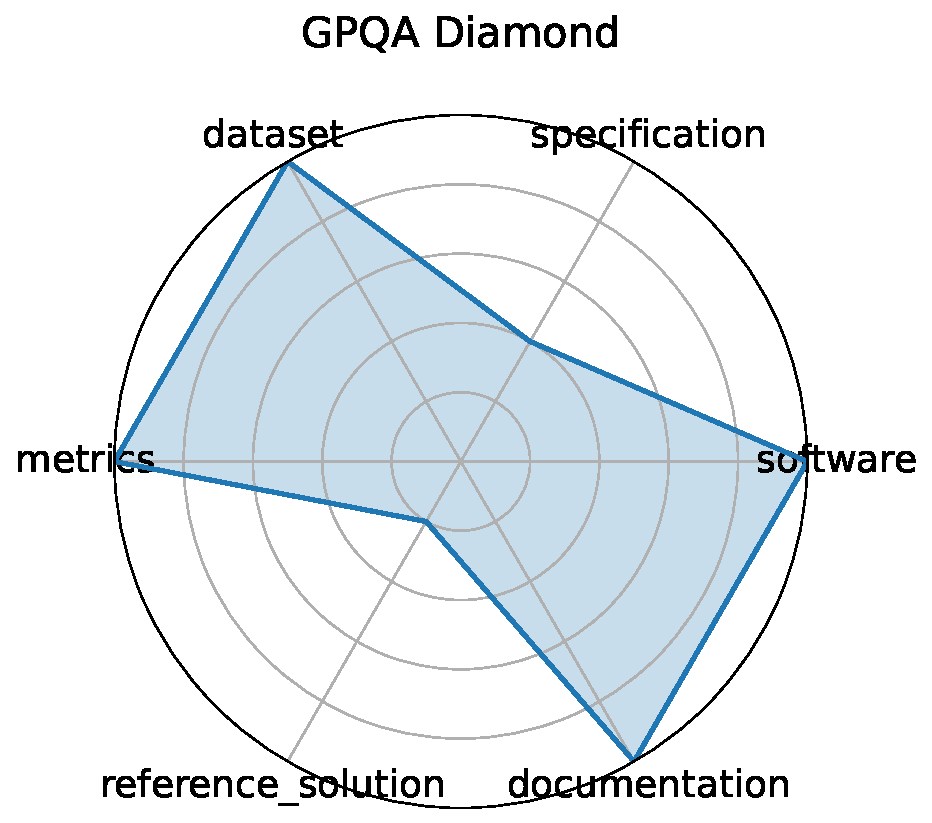
\includegraphics[width=0.2\textwidth]{gpqa_diamond_radar.pdf}
}}
\clearpage